\documentclass[]{article}


%-----------------------------------------------------------------------------------------------------------------------------------------
%
%   GLOBALS
%
%-----------------------------------------------------------------------------------------------------------------------------------------
\newcommand{\DOCTITLE}{

}
\newcommand{\DOCAUTHOR}{

}
\newcommand{\DISCLAIMER}
{
    \topskip0pt
    \vspace*{\fill}
    {
    \centering
        \small{
            THIS DOCUMENT IS INTENDED FOR INTERNAL USE ONLY
        }
    }
    \\
    {
    \centering
        \small{
        UNAUTHORIZED DISTRIBUTION OF THIS DOCUMENT IS STRICTLY PROHIBITED 
        }
    }
    \vspace*{\fill}
}

\usepackage{lmodern}
\usepackage{amssymb,amsmath}
\usepackage{ifxetex,ifluatex}
\usepackage{fixltx2e} % provides \textsubscript
\ifnum 0\ifxetex 1\fi\ifluatex 1\fi=0 % if pdftex
  \usepackage[T1]{fontenc}
  \usepackage[utf8]{inputenc}
\else % if luatex or xelatex
  \ifxetex
    \usepackage{mathspec}
    \usepackage{xltxtra,xunicode}
  \else
    \usepackage{fontspec}
  \fi
  \defaultfontfeatures{Mapping=tex-text,Scale=MatchLowercase}
  \newcommand{\euro}{€}
\fi
% use upquote if available, for straight quotes in verbatim environments
\IfFileExists{upquote.sty}{\usepackage{upquote}}{}
% use microtype if available
\IfFileExists{microtype.sty}{%
\usepackage{microtype}
\UseMicrotypeSet[protrusion]{basicmath} % disable protrusion for tt fonts
}{}
\ifxetex
  \usepackage[setpagesize=false, % page size defined by xetex
              unicode=false, % unicode breaks when used with xetex
              xetex]{hyperref}
\else
  \usepackage[unicode=true]{hyperref}
\fi
\usepackage[usenames,dvipsnames]{color}
\hypersetup{breaklinks=true,
            bookmarks=true,
            pdfauthor={},
            pdftitle={},
            colorlinks=true,
            citecolor=blue,
            urlcolor=blue,
            linkcolor=magenta,
            pdfborder={0 0 0}}
\urlstyle{same}  % don't use monospace font for urls
\usepackage{biblatex}
\addbibresource{bibliography.bib}
\usepackage{graphicx,grffile}
\makeatletter
\def\maxwidth{\ifdim\Gin@nat@width>\linewidth\linewidth\else\Gin@nat@width\fi}
\def\maxheight{\ifdim\Gin@nat@height>\textheight\textheight\else\Gin@nat@height\fi}
\makeatother
% Scale images if necessary, so that they will not overflow the page
% margins by default, and it is still possible to overwrite the defaults
% using explicit options in \includegraphics[width, height, ...]{}
\setkeys{Gin}{width=\maxwidth,height=\maxheight,keepaspectratio}
\usepackage[normalem]{ulem}
% avoid problems with \sout in headers with hyperref:
\pdfstringdefDisableCommands{\renewcommand{\sout}{}}
\setlength{\parindent}{0pt}
\setlength{\parskip}{6pt plus 2pt minus 1pt}
\setlength{\emergencystretch}{3em}  % prevent overfull lines
\providecommand{\tightlist}{%
  \setlength{\itemsep}{0pt}\setlength{\parskip}{0pt}}
\setcounter{secnumdepth}{0}

\date{}

% Redefines (sub)paragraphs to behave more like sections
\ifx\paragraph\undefined\else
\let\oldparagraph\paragraph
\renewcommand{\paragraph}[1]{\oldparagraph{#1}\mbox{}}
\fi
\ifx\subparagraph\undefined\else
\let\oldsubparagraph\subparagraph
\renewcommand{\subparagraph}[1]{\oldsubparagraph{#1}\mbox{}}
\fi

%-----------------------------------------------------------------------------------------------------------------------------------------
%
%   PAGE SIZE AND MARGINS
%
%-----------------------------------------------------------------------------------------------------------------------------------------
\usepackage[a4paper,headheight=30pt]{geometry}
%\usepackage[letterpaper, portrait, margin=2in]{geometry}
\addtolength{\topmargin}{-.5in}
\addtolength{\textheight}{1.75in}

\usepackage{graphicx}

\usepackage{fancyhdr}
\pagestyle{fancy}


%-----------------------------------------------------------------------------------------------------------------------------------------
% Page break after sections
%-----------------------------------------------------------------------------------------------------------------------------------------
%\usepackage{titlesec}
%\newcommand{\sectionbreak}{\clearpage}

\lhead{
    %left header content
%    \topskip0pt
%    \vspace*{\fill}
    {
    \centering
        
\includegraphics[height=2.66em]{template/sc.png}
    }
%    \vspace*{\fill}
}
\chead{
    \topskip0pt
    \vspace*{\fill}
    {
    \centering
        \small{
            THIS DOCUMENT IS INTENDED FOR INTERNAL USE ONLY
        }
    }
    \\
    {
    \centering
        \small{
        UNAUTHORIZED DISTRIBUTION OF THIS DOCUMENT IS STRICTLY PROHIBITED 
        }
    }
    \vspace*{\fill}
}
\rhead{
%    \topskip0pt
%    \vspace*{\fill}
    % right header content
    {
    \centering
        
\includegraphics[height=3.25em]{template/scrd.png}
    }
%    \vspace*{\fill}
}
\lfoot{
    % left footer content
    \topskip0pt
    \vspace*{\fill}
    SCRD
    Revision 0.1
    \vspace*{\fill}
}
\cfoot{
    % middle footer content
    \topskip0pt
    \vspace*{\fill}
    {
    \centering
    SCRD Internal Documents Template \\
    \today
    }
    \vspace*{\fill}
}
\rfoot{
    % right footer content
    \topskip0pt
    \vspace*{\fill}
    \thepage
    \vspace*{\fill}
}
% extend the header into the margins
\usepackage{calc}
\fancyheadoffset[L,R]{\marginparsep+\marginparwidth}

%--------------------------------------------------------------------------------------------------------------
%	My Packages
%--------------------------------------------------------------------------------------------------------------
\usepackage{capt-of}

%--------------------------------------------------------------------------------------------------------------
%
%	BEGIN DOCUMENT
%
%--------------------------------------------------------------------------------------------------------------
\begin{document}


%--------------------------------------------------------------------------------------------------------------
%
%	TITLE PAGE
%
%--------------------------------------------------------------------------------------------------------------
\begin{titlepage}

\newcommand{\HRule}{\rule{\linewidth}{0.5mm}} % Defines a new command for the horizontal lines, change thickness here

\center % Center everything on the page
 
%----------------------------------------------------------------------------------------
%	HEADING SECTIONS
%----------------------------------------------------------------------------------------

\includegraphics[width=200pt,height=200pt]{../images/rocketry_logo_large.png}\\[1cm] % Include a department/university logo - this will require the graphicx package
\textsc{\Large Space Concordia - Rocketry Division}\\[0.5cm] % Major heading such as course name
\textsc{\large Aurelius CR-2-4G - Structural Team}\\[0.5cm] % Minor heading such as course title

%----------------------------------------------------------------------------------------
%	LOGO SECTION
%----------------------------------------------------------------------------------------

\begin{figure}[ht]
    \centering
    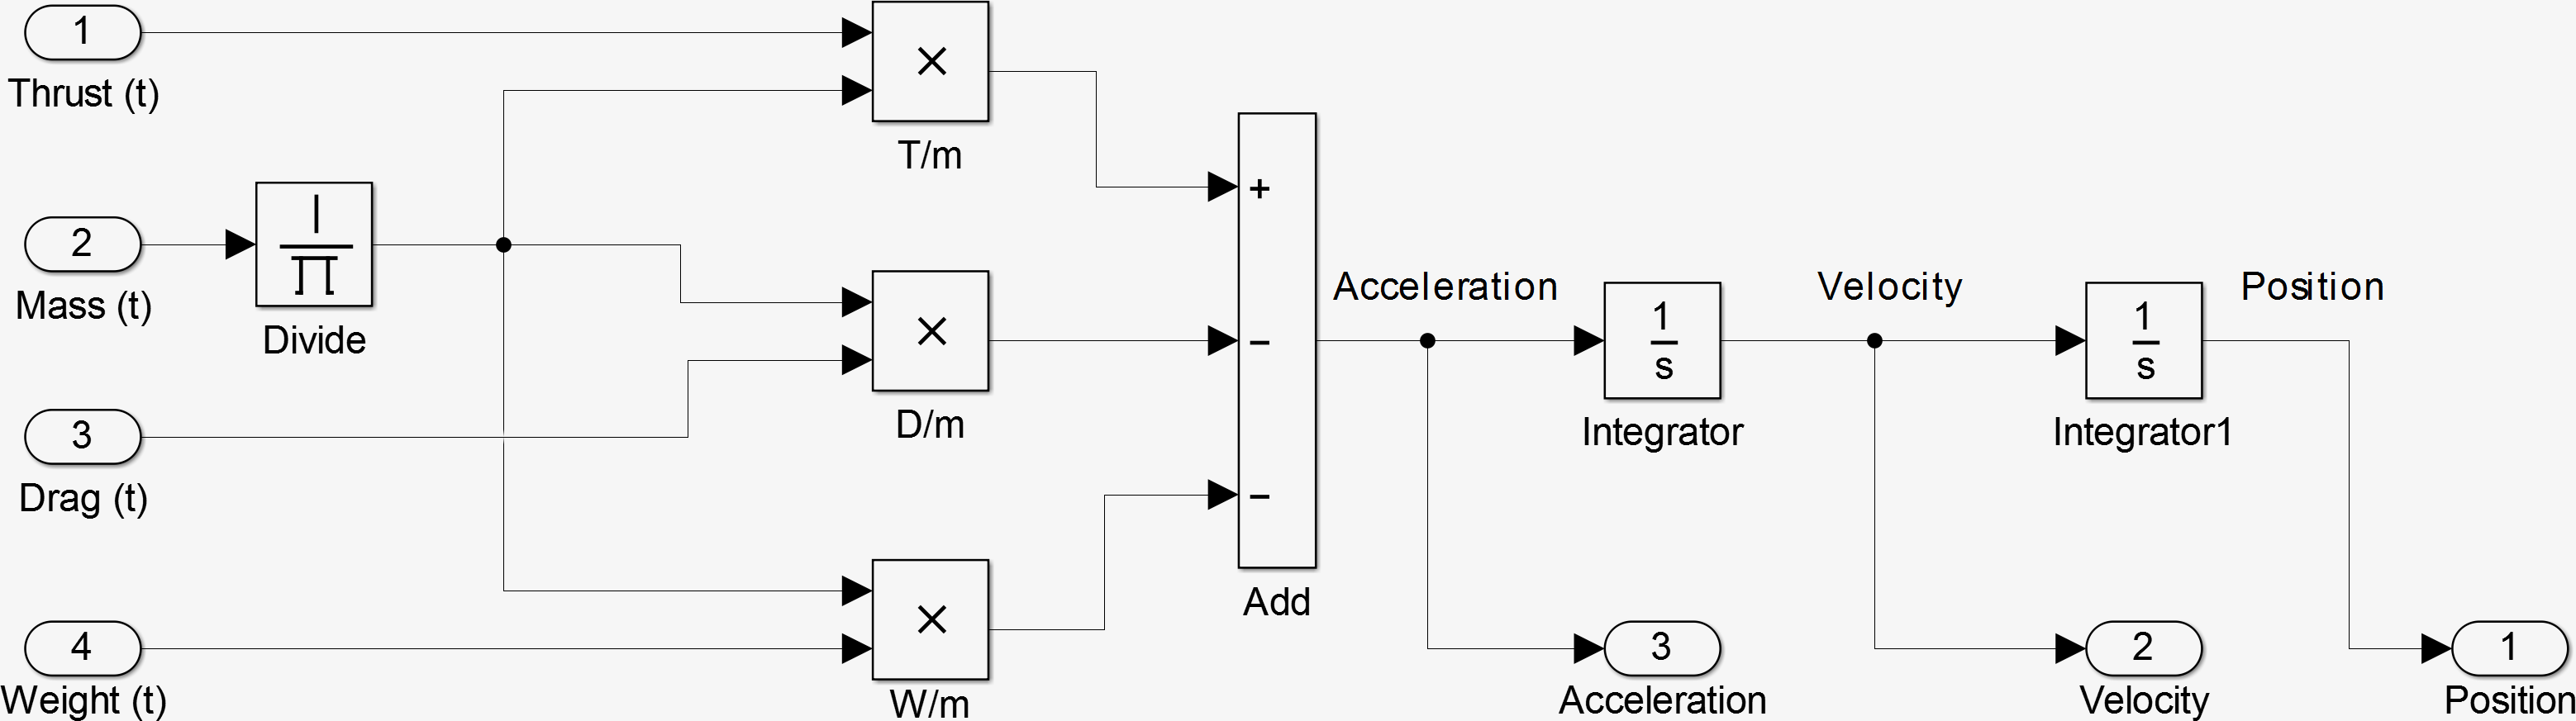
\includegraphics[height=100pt]{../images/vertical_model_simplified.png}\\
\end{figure}

%----------------------------------------------------------------------------------------
%	TITLE SECTION
%----------------------------------------------------------------------------------------

\HRule \\[0.6cm]
{ \Huge \bfseries 
Performance Model Specification
}\\[0.4cm] 

\HRule \\[1cm]
 
%----------------------------------------------------------------------------------------
%	AUTHOR SECTION
%----------------------------------------------------------------------------------------

\begin{minipage}{0.4\textwidth}
\begin{flushleft} \large
	\begin{tabular} {r l} 
        \emph{Author(s):} & Shawn Bulger	\\
	\end{tabular}
\end{flushleft}
\end{minipage}
~
\begin{minipage}{0.4\textwidth}
\begin{flushright} \large
	\begin{tabular} {r l} 
		\emph{Coordinator:} & Dr. Ashok Kaushal 		\\
		\emph{Supervisor:}  & Dr. Mehdi Hojjati 		\\
		\emph{EIR:}         & Dominic Ng  		        \\
	\end{tabular}
\end{flushright}
\end{minipage}\\[2cm]

%----------------------------------------------------------------------------------------
%	DATE SECTION
%----------------------------------------------------------------------------------------

{\large \today}\\[2cm] % Date, change the \today to a set date if you want to be precise

\vfill % Fill the rest of the page with whitespace

\end{titlepage}

{
\hypersetup{linkcolor=black}
\setcounter{tocdepth}{3}
\tableofcontents
\clearpage
}
\listoftables
\listoffigures
\clearpage
\section{Arcturus Analysis}\label{arcturus-analysis}

\subsection{Competition Results}\label{competition-results}

\subsubsection{Analysis on 2015/07/23}\label{analysis-on-20150723}

\begin{itemize}
\tightlist
\item
  custom avionics registered altitude of 15,000 ft
\item
  commercial avionics registered altitude of 12,700 ft
\item
  using most accurate simulation data available:

  \begin{itemize}
  \tightlist
  \item
    rocket could not have exceeded 11,000 ft
  \item
    when avionics were tested in smaller rocket, they returned accurate
    values
  \end{itemize}
\end{itemize}

\subsubsection{Analysis on 2015/07/28}\label{analysis-on-20150728}

\begin{itemize}
\tightlist
\item
  analysis of the StrattoLogger Data shows that the temperature inside
  the avionics bay did not decrease as expected, throwing off the sound
  speed calculations
\item
  reviewing the `hyposometric' formula being used (think it should read
  `hypsometric')
\end{itemize}

\paragraph{Theories}\label{theories}

\begin{itemize}
\tightlist
\item
  \sout{latent heat and pressure built up in avionics bay while on
  launch pad in hot desert environment}

  \begin{itemize}
  \tightlist
  \item
    we now suspect that the air is being vented and that there is not a
    build up of pressure in the avionics bay
  \end{itemize}
\item
  we rather suspect that the rocket structure is heating up the air
  inside, causing the false readings
\item
  it seems possible that there are issues with the `hyposometric'
  formula
\item
  Robert Winchcomb suggested that a power fluctuation could be the cause
  of the anomalous bump in the velocity data
\end{itemize}

\paragraph{Action Taken}\label{action-taken}

\begin{itemize}
\tightlist
\item
  beginning to plot the data to help confirm our suspicions
\item
  may need to consider thermal control aspects to solve this problem
\end{itemize}

\clearpage

\subsection{Altitude Determination}\label{altitude-determination}

\subsection{Resources}\label{resources}

\begin{itemize}
\tightlist
\item
  it seems the previous team used the following resource to determine
  altitude
\item
  \href{http://forum.arduino.cc/index.php?topic=261589.0}{Arduino Forum
  Post 261589}
\item
  \href{http://glossary.ametsoc.org/wiki/Hypsometric_equation}{Meterology
  Glossary - Hypsometric Equation}
\end{itemize}

\subsection{Deriving the correct hypsometric
equation}\label{deriving-the-correct-hypsometric-equation}

\[ P_{actual} = (P_o + P_{dev}) * \left[(1-0.0065* \left( \dfrac{ altitude } { T_o + T_{dev} } \right) \right]^{5.2561} \]

\[ \dfrac{P_{actual}}{ (P_o + P_{dev})  } = \left[(1-0.0065* \left( \dfrac{ altitude } { T_o + T_{dev} } \right) \right]^{5.2561} \]

\[ 
\left( \dfrac{ P_{actual} }{ (P_o + P_{dev}) } \right)^{( 1/5.2561 )} 
= 
1-0.0065 \cdot \left( \dfrac{ altitude } { T_o + T_{dev} } \right) 
\]

\[ 
1 - \left( \dfrac{ P_{actual} }{ (P_o + P_{dev}) } \right)^{( 1/5.2561 )} 
= 
0.0065 \cdot \left( \dfrac{ altitude } { T_o + T_{dev} } \right) 
\]

\[ 
\dfrac{ \left( T_o + T_{dev} \right) \left( 1 - \left( \dfrac{ P_{actual} }{ (P_o + P_{dev}) } \right)^{( 1/5.2561 )} \right) } { \left( 0.0065 \right) }
= 
altitude 
\]

\begin{equation}
\label{eq_hyposometric_altitude}
altitude=
\dfrac{ \left( T_o + T_{dev} \right) \left( 1 - \left( \dfrac{ P_{actual} }{ (P_o + P_{dev}) } \right)^{( 1/5.2561 )} \right) } { \left( 0.0065 \right) }
\end{equation}

Equation (\ref{eq_hyposometric_altitude}) above seems equivalent to the
form used in avionics code (Equation
(\ref{eq_hyposometric_altitude_avionics}) below)

\begin{equation}
\label{eq_hyposometric_altitude_avionics}
altitude =
\dfrac{ \left( T_o + T_{dev} \right) \left( \left( \dfrac{ (P_o + P_{dev}) }{ P_{actual} } \right)^{( 1/5.2561 )}  - 1 \right) } { \left( 0.0065 \right) }
\end{equation}

\clearpage

\subsection{Analysis}\label{analysis}

\subsubsection{Custom Avionics Accelerometer
Data}\label{custom-avionics-accelerometer-data}

In Figure \ref{arcturus_accelerometer_plot_label} below, the
accelerometer data is plotted. The Longitudinal and Vertical axis is the
X-axis. Unfortunately the sensor was not calibrated correctly, and the
force curve is clipped at 2 Gs. We expect that the rocket experienced up
to 10 or 11 Gs. If we were able to capture the entire force curve, we
could infer the drag force experienced by the rocket to compare with our
simulation results.

\begin{figure}[htbp]
\centering
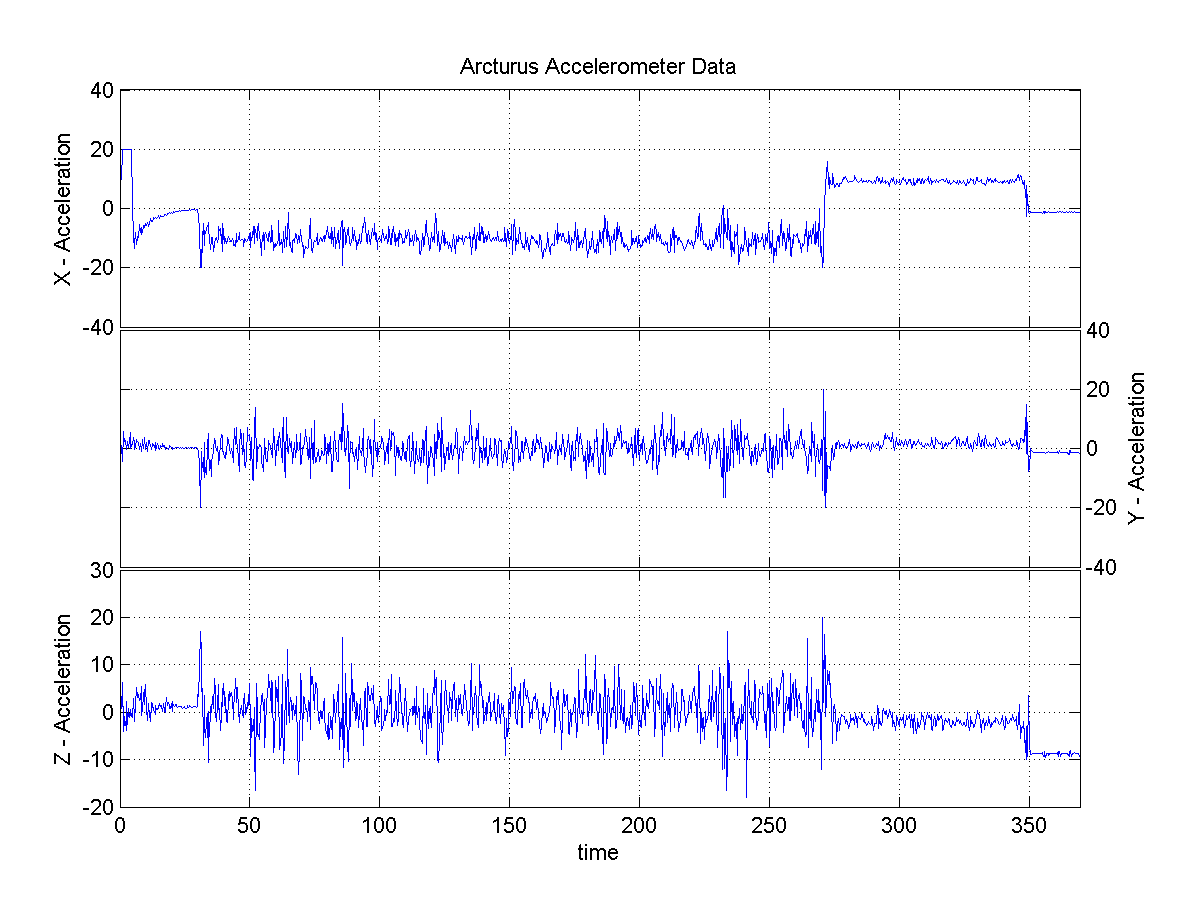
\includegraphics{images/plots/arcturus_accelerometer_plot.png}
\caption{X, Y, and Z acceleration a Function of Time
\label{arcturus_accelerometer_plot_label}}
\end{figure}

Figure \ref{arcturus_accelerometer_apogee_plot_label} below shows the
longitudinal acceleration during the approach to apogee. We can see the
peak in force along the X-axis, with a sudden step down to roughly
negative 17 \(m/s^2\), as the drag force coupled with the force of
gravity steeply decelerates the rocket.

This negative region can be used to analyze a segment of the flight
curve approaching apogee.

\begin{figure}[htbp]
\centering
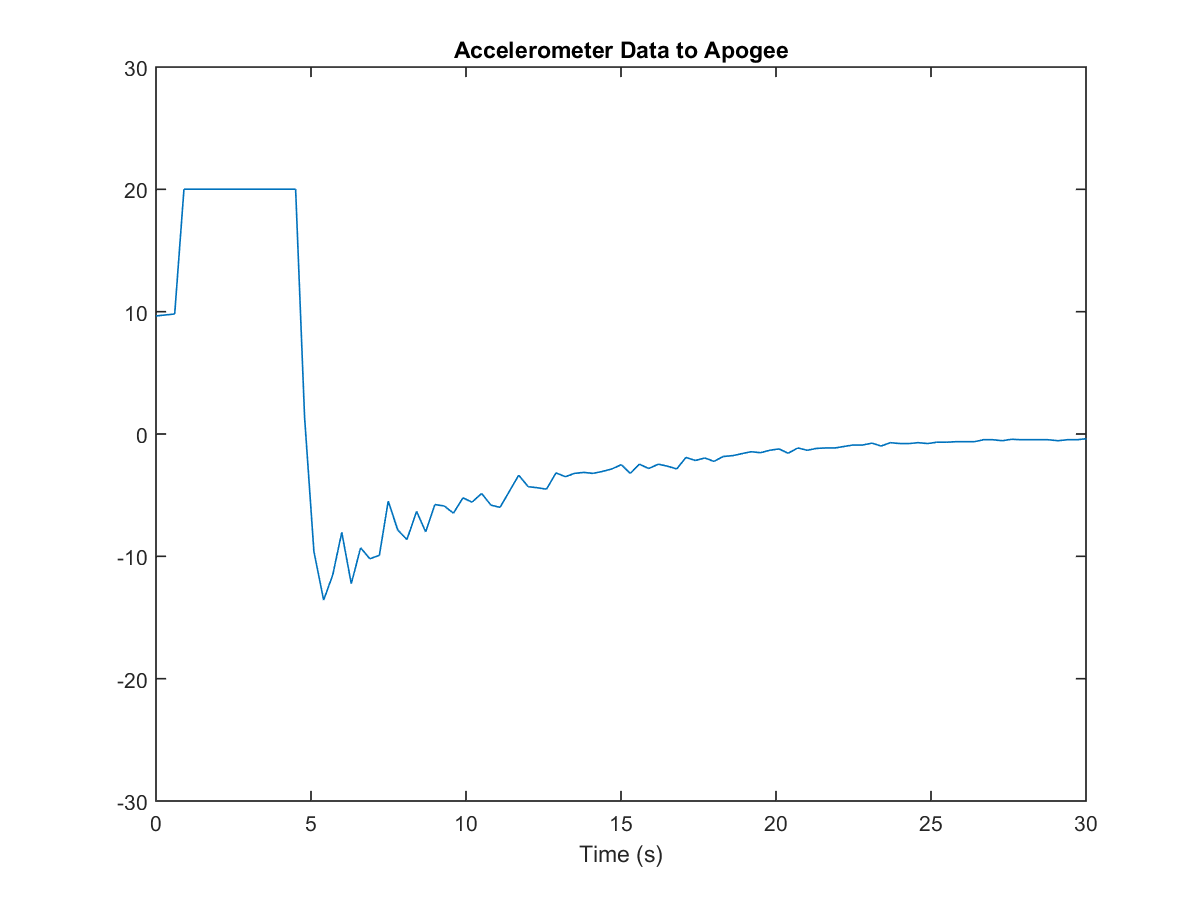
\includegraphics{images/plots/arcturus_accelerometer_apogee_plot.png}
\caption{Longitudinal Acceleration as a Function of Time
\label{arcturus_accelerometer_apogee_plot_label}}
\end{figure}

\clearpage

\subsubsection{Custom Avionics Barometric Sensor
Data}\label{custom-avionics-barometric-sensor-data}

\begin{figure}[htbp]
\centering
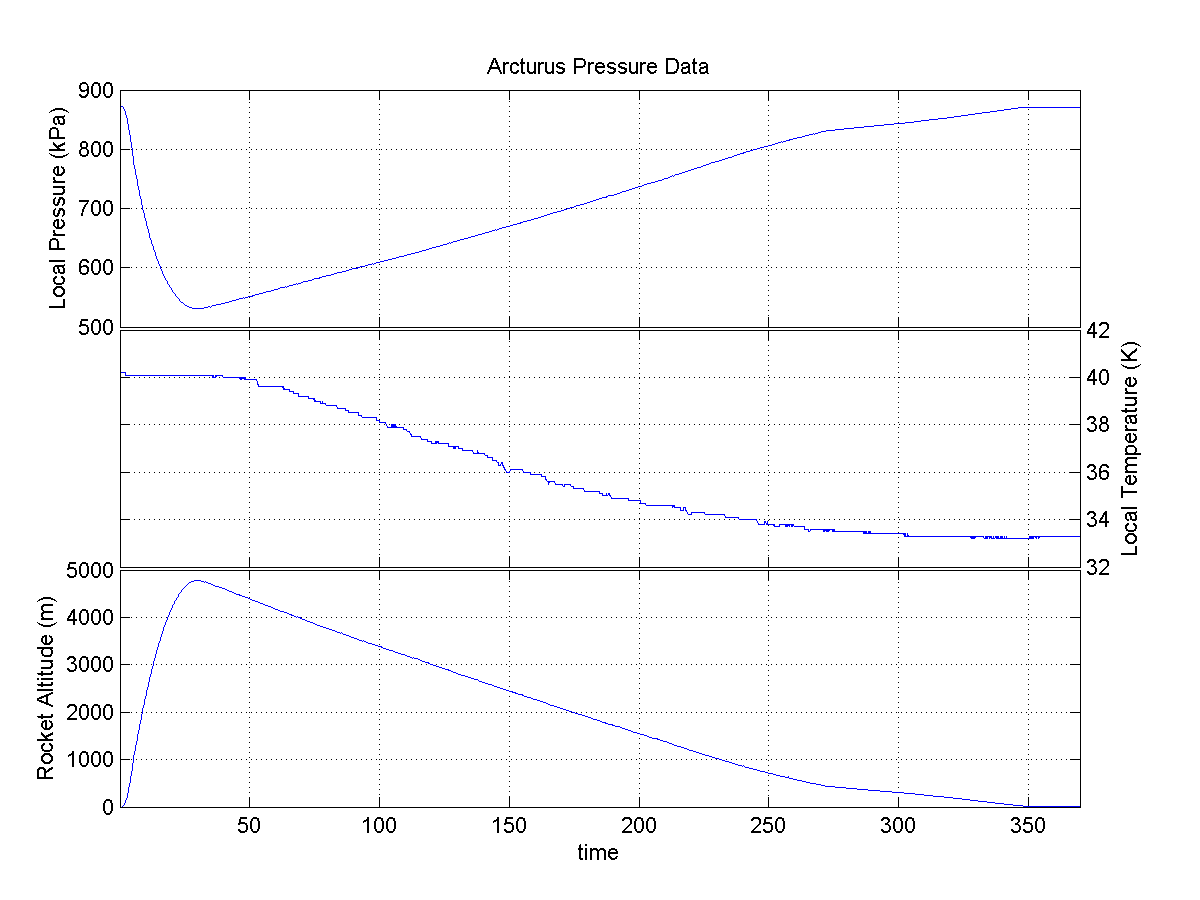
\includegraphics{images/plots/arcturus_pressure_plot.png}
\caption{Pressure, Temperature, Altitude as a function of time
\label{arcturus_pressure_plot_label}}
\end{figure}

\clearpage

Figure \ref{arcturus_strattologger_plot_label} below shows the data
acquired from the Commercial Stratologger altimeter provided by
\emph{Perfect Flight}. Velocity and acceleration data is apparently
derived from the altitude as a function of time
\href{https://www.apogeerockets.com/Electronics_Payloads/Altimeters/PerfectFlite_StratoLogger_Altimeter}{ApogeeRockets
Link}

\subsubsection{Commercial Stratologger
Data}\label{commercial-stratologger-data}

\begin{figure}[htbp]
\centering
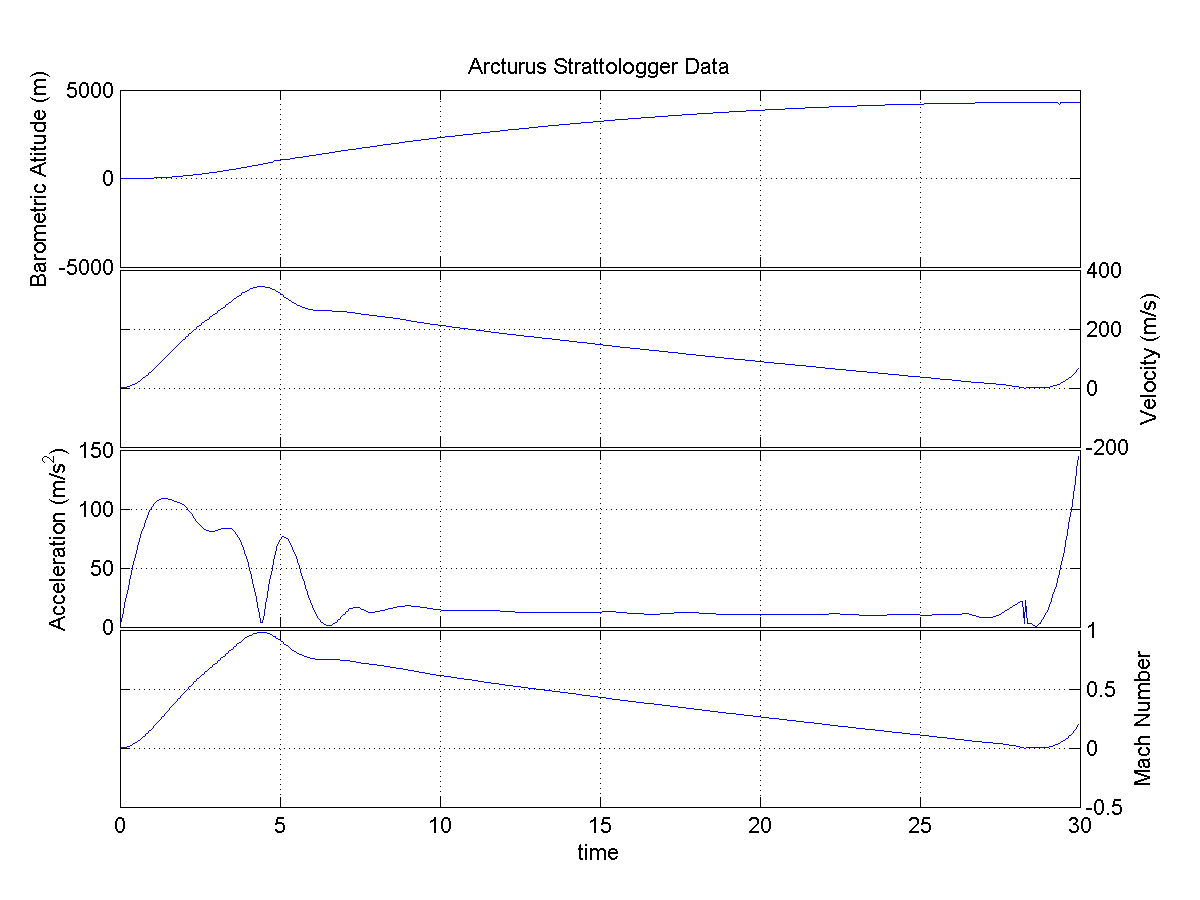
\includegraphics{images/plots/arcturus_strattologger_plot.png}
\caption{Altitude, Velocity, Acceleration, and Mach Number as a function
of time \label{arcturus_strattologger_plot_label}}
\end{figure}

\clearpage

\subsubsection{OpenRocket Simulation
Data}\label{openrocket-simulation-data}

\begin{figure}[htbp]
\centering
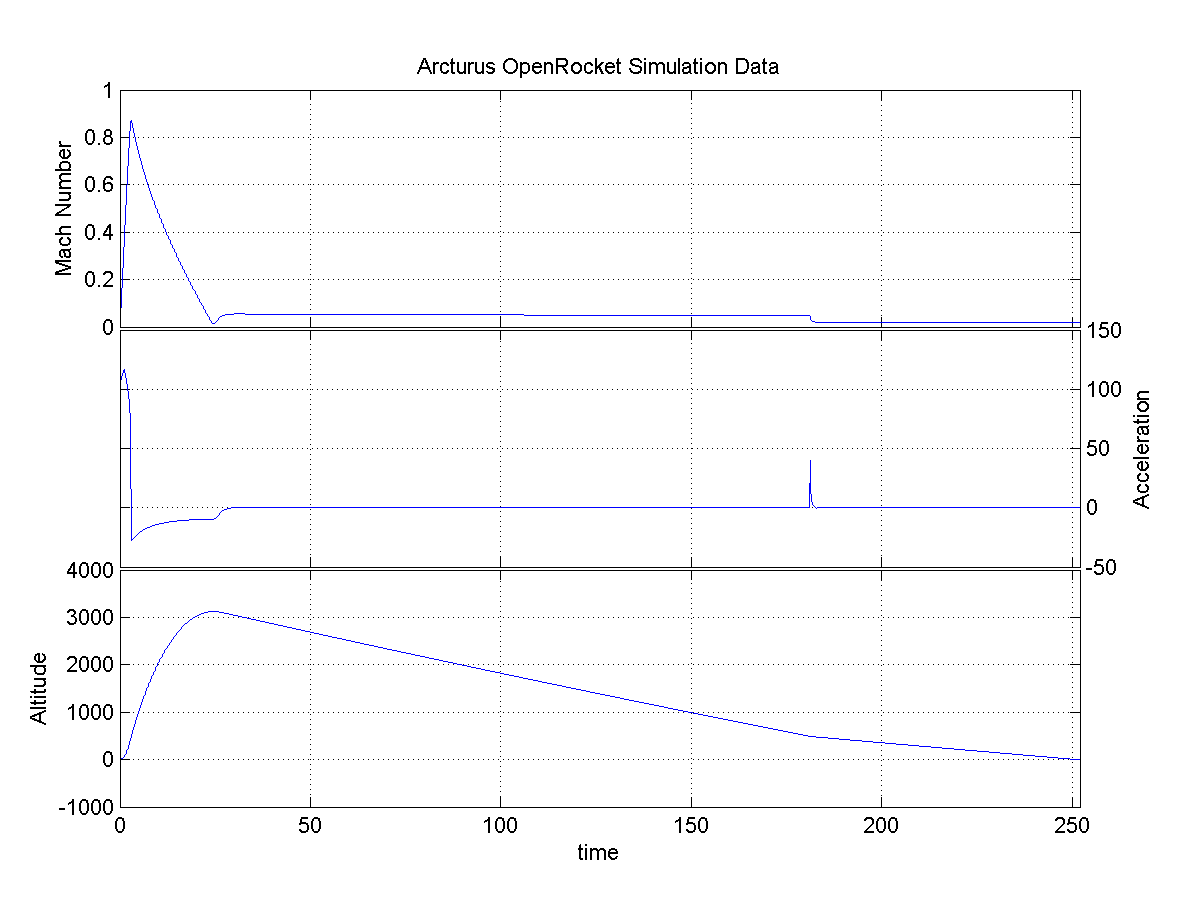
\includegraphics{images/plots/arcturus_openrocket_plot.png}
\caption{Altitude, Acceleration, and Mach Number as a function of time
\label{arcturus_openrocket_plot_label}}
\end{figure}

\clearpage

\printbibliography

\end{document}
